%% INCOM 2027 -- invited session "From Supply Chain to Shop Floor: Trustworthy AI for Resilient Decision-Making
%% under Disruption". Draft. Compile with the IFAC template (ifacconf.cls, ifacconf.bst), e.g. on Overleaf.
%% Every number in this file comes from the repository's result files (see paper/README.md for the mapping).
\documentclass{ifacconf}

\usepackage{graphicx}
\usepackage{natbib}
\usepackage{amsmath,amssymb}
\usepackage{booktabs}
\usepackage{eurosym}
\usepackage{siunitx}
\sisetup{group-separator={,},group-minimum-digits=4}

\begin{document}
\begin{frontmatter}

\title{Predict, decide, explain, certify: trustworthy disruption response on an evidence-based supply-chain twin}

% TODO(authors): confirm the author list, order and e-mail addresses.
\author[First]{Ahmad Salameh}
\author[First]{Sara Himmiche}

\address[First]{SYMME, Universit\'e Savoie Mont Blanc, Annecy, France}

\begin{abstract}
AI layers on supply-chain digital twins are usually trained and assessed on one calibrated simulator. We ask
what such layers can be trusted to do when every part of the twin, and every disruption injected into it, is
backed by data, and when they are tested on a team they were not built on. From the SAP data of three ERPsim game
years played on the same company we derive and validate a day-level twin, generated identically in Python and as
an UPPAAL model. Disruptions are sampled within open-data and in-game evidence, and responses use only the levers
the human players had. Four layers predict the impact of a notified disruption with conformal bounds, choose a
response under a service constraint, distil the choice into a readable tree, and certify it with
Clopper--Pearson and statistical model checking. In the build year the certified tree raises the service level
from 75.7\,\% to at least 78.2\,\% with at most 2.0\,\% harm. On other teams' years, coverage, decision value and
certificates degrade unless the layers are recalibrated or adapted on the target twin.
\end{abstract}

\begin{keyword}
Digital twin; supply chain resilience; disruption management; conformal prediction; statistical model checking;
explainable AI; ERP data.
\end{keyword}

\end{frontmatter}

%% ------------------------------------------------------------------------------------------------------------
\section{Introduction}

Disruptions of supply, production and demand propagate through stock and capacity into lost sales, and
decision support for them is increasingly built as AI layers on top of digital twins
\citep{ivanov2021digitaltwin,baryannis2019scrm}. Whether such support can be trusted depends on two things that
are rarely examined together. The first is the twin: an AI layer can only be as credible as the simulator it
learns from and is checked against, yet twins are often calibrated quickly to whatever data exists and validated,
if at all, on the data used to build them \citep{sargent2013vv}. The second is the AI layer itself: its
predictions, its decisions and its explanations should come with statements of how often they hold, for the
situations in which they will actually be used.

This paper builds both from the same evidence. The twin is derived from the SAP tables of an ERPsim
manufacturing game \citep{leger2006erpsim} released as open research data \citep{tritscher2022openerp}. Three game
years of one company, played by teams with different policies, provide a natural test of transfer: everything is
built on one year and checked on the other two. On this twin we stack four layers --- predict, decide, explain,
certify --- and report where they hold and where they do not (Fig.~\ref{fig:framework}).

The contributions are:
(i) an \emph{evidence-first} twin: every parameter, structural rule and player decision is derived from the
recorded data, validated against two unseen years under a pre-registered protocol, and generated as both a Python
simulator and an UPPAAL model that agree in 591 of 591 deterministic configurations;
(ii) disruptions sampled \emph{within evidence bounds} (open shipment data and the game's own scrap and stoppage
records) and responses restricted to the levers the players had;
(iii) a predict--decide--explain--certify pipeline whose decision rule is constrained by conformal bounds and
whose certified object is the explanation itself; and
(iv) a measured account of transfer: the layers work in their build year, degrade on another team's year, and
recover with recalibration or adaptation on the target twin, while explanation stability does not reveal the
degradation.

\begin{figure*}[t]
\centering
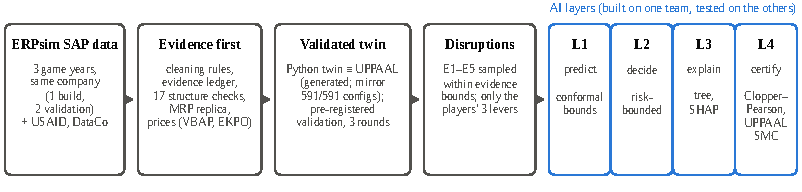
\includegraphics[width=\textwidth]{figures/fig1_framework.pdf}
\caption{Evidence-first pipeline: every model element is derived from the SAP data of one game year and checked on
two years played by another team; the Python twin and the generated UPPAAL model agree in 591 of 591 deterministic
configurations; disruptions are sampled within evidence bounds and the AI layers may use only the players' levers.}
\label{fig:framework}
\end{figure*}

%% ------------------------------------------------------------------------------------------------------------
\section{Related work}

Digital twins for supply chain resilience range from discrete-event models of disruption propagation to
optimisation-based recovery \citep{ivanov2021digitaltwin,hosseini2019resilience}, and AI is used for risk
prediction and response \citep{baryannis2019scrm}. Most studies use one calibrated simulator and report average
performance. Conformal prediction gives distribution-free coverage under exchangeability
\citep{vovk2005alrw,romano2019cqr,angelopoulos2023gentle}; its behaviour under covariate shift has been studied
through importance weighting \citep{tibshirani2019covariateshift} and online adaptation \citep{gibbs2021aci}.
Interpretable policies can be obtained by distilling a black box into a tree \citep{bastani2017extraction} and
are preferable in high-stakes settings \citep{rudin2019stop}; for controllers, decision-tree representations are
established in formal methods \citep{ashok2020dtcontrol}. Statistical model checking estimates the probability of
temporal properties with confidence bounds \citep{legay2010smc}; UPPAAL SMC and Stratego support stochastic hybrid
models and strategy synthesis \citep{david2015uppaalsmc,david2015stratego}, and SMC has been used to evaluate the
robustness of production schedules \citep{himmiche2018smc}. Our work combines these elements on a twin whose
evidence base and validation are part of the contribution, and tests transfer across real policy shifts.

%% ------------------------------------------------------------------------------------------------------------
\section{An evidence-first twin}

\subsection{Data}
ERPsim runs a simulated company in SAP; each round of the game spans 20 simulated days and a year has 12 rounds.
The released data \citep{tritscher2022openerp} contain several game years, some with labelled fraud cases. We use
the three years of one player group: \emph{normal~2} (build year) and \emph{fraud~2}, \emph{fraud~3} (validation
years); the fraud-labelled documents are excluded from demand statistics. The company sells one detailed product
(F12) to about 70 customers through three distribution centres (DCs), makes it with five of eight components
(food and packaging) on a production line of \num{24000} units per day shared with two to three other products, and
buys components with lead times of mostly one to six days.

\subsection{Evidence ledger, structure and policy}
Every element is derived by scripts from the SAP tables and recorded with its source, method and value in each
year. Seventeen structural claims are tested in all three years, among them: unmet demand is lost (no backorders),
each customer is served by one DC, plant-to-DC transfers are instantaneous, all products share one line, an order
starts only when components for its whole batch are in stock (78 of 78 recorded starts), the mass balance closes,
and the game starts with empty stock. The players' only planning decision is the forecast; SAP MRP turns it into
production and purchase orders, and an MRP replica reproduces 20 of 21 production decisions and 29 of 37 purchasing
runs. Component purchase prices (EKPO) and sales prices (VBAP) give a margin of 1.81 to 2.37\,\euro{} per unit.

\subsection{Twin and validation}
The twin advances in daily steps (one time unit is one game day): supplier receipts, production on the shared
line with a 0.6-day changeover, plant-to-DC transfers, sales clipped to DC stock, and decisions. For validation the
players' recorded decisions are replayed, so that the test concerns the physics. A protocol fixed on the build
year before the validation years were run defines a primary cumulative-deviation metric (A1) and secondary metrics
on stock-out months, planning delay, component stock-outs and a recorded production pause. Two later amendments are
disclosed. The latest (round~3) replays a transfer that cannot ship for lack of plant stock as soon as stock allows:
plain replay had left the clipped part at the plant for ever, holding two to four times the recorded plant stock.
With this rule, yearly sales are within 1\,\% of the record in all three years and transfers are exact (A1 for
sales 0.5, 1.0 and 1.0\,\%; for transfers 2.2, 3.6 and 2.1\,\%). Normal~2 fails one secondary metric, fraud~2 two
and fraud~3 four. A data-only check traces the fraud-year stock-out differences to a constant offset of about two
days of demand per DC, created by first-month losses that the recorded (censored) demand cannot reproduce; fraud~3
also contains fraud orders that physically removed \num{67431} units. The pre-registered verdict is therefore not
met for fraud~3, which we use only as a shift test.

\subsection{One twin, two implementations}
An UPPAAL model is generated from the same inputs: one day-tick timed automaton whose step function executes the
same day, with all quantities as doubles so that the arithmetic matches. With every lead time at its median the
model is deterministic, and a line-by-line Python transcription of the generated file reproduces the twin day by
day in 591 of 591 configurations (all disruption types, all response actions and the decision tree of
Section~\ref{sec:explain}; maximum difference $10^{-10}$ units). Running the generated files in \texttt{verifyta}
is the remaining check (Section~\ref{sec:discussion}).

%% ------------------------------------------------------------------------------------------------------------
\section{Disruptions within evidence, and the levers}

A disruption is admitted only if it acts through a mechanism of the validated physics and its severity comes from
evidence (Table~\ref{tab:disruptions}); open-data evidence is transferred only as dimensionless ratios. Each
disruption starts at a random day of the steady months, because its impact depends strongly on where it falls
relative to the production queue.

\begin{table*}[t]
\caption{Disruptions, their mechanism in the twin, and the evidence for their severity.}
\label{tab:disruptions}
\centering\small
\begin{tabular}{@{}p{2.4cm}p{6.4cm}p{8.2cm}@{}}
\toprule
Disruption & Mechanism & Severity range (evidence)\\
\midrule
E1 supplier delay & POs created in a 20-day window arrive $\lceil r\,\ell\rceil$ days late &
$r \le 0.96$: delay/lead time of late shipments, USAID SCMS \citep{usaid_scms} (\num{10324} shipments)\\
E2 quality loss & share $b$ of receipts blocked and re-ordered; the rest 2 days late &
$b \in [0.2, 4.1]\,\%$: the game's six scrap events\\
E3 line stoppage & the shared line stops for $n$ days & $n \le 25$: shortest recorded production pause\\
E4 demand surge & demand $\times f$ for 20 days & $f \le 1.19$: build-year monthly range\\
E5 transit delay & plant-to-DC shipments arrive $k$ days late & $k \le 4$: DataCo q95 \citep{dataco2019}, an upper bound\\
\bottomrule
\end{tabular}
\end{table*}

Under the players' own decisions the same disruption hits the three teams very differently: a one-month
19\,\% surge costs normal~2 a median of \num{28296} extra lost units, fraud~2 \num{5915} and fraud~3 none, and a
25-day stoppage costs \num{54531}, \num{13363} and \num{19324} units. Supplier and quality disruptions have a
median impact of zero in every year: the players' buffers absorb them except at unlucky timings (13--27\,\% of runs
in normal~2). Resilience is thus a property of the policy state, which motivates layers that observe it.

Responses may use only the players' levers: purchase orders (a component buffer of 5 or 10 days of recent
consumption), production-order conversions (an extra F12 batch of one line-day, or F12 priority on the line by
holding other products' conversions while F12 waits) and transfers (rebalancing DCs by days of cover). With
combinations these form eight actions, including ``no response''. The cost of an action is the extra inventory
capital it ties up, valued at material cost; no holding-cost rate is assumed. Because the line runs at 82--93\,\%
load, giving F12 priority moves loss to the other products, so the objective counts the lost demand of all
products.

%% ------------------------------------------------------------------------------------------------------------
\section{Predict, decide, explain, certify}

\subsection{Episodes}
An episode is a game year, a start day, a seed and a disruption drawn within Table~\ref{tab:disruptions}. The twin
runs it once without the disruption and once under the disruption for each action, with common random numbers.
The features are what a planner observes at the notice (component cover, the production queue, plant and DC
cover, recent losses, the transfer backlog, and the notice's type and severity), recorded inside the run so that
no future information leaks; all are dimensionless because the years run at different demand levels. We generate
\num{2000} episodes per year, 600 per year with severities beyond the evidence (STRESS), and an independent
certification sample of \num{2000} build-year episodes. All layers are built on normal~2 (60\,\% training,
20\,\% calibration) and tested on its held-out 20\,\%, on fraud~2 and fraud~3, and on STRESS.

\subsection{L1: predict}
The target is the extra lost demand over the 60 days after the notice, in days of demand. A gradient-boosted \citep{ke2017lightgbm}
quantile model $\hat q(x)$ at level $1-\alpha=0.9$ is corrected by split conformal prediction: with calibration
scores $s_i = y_i - \hat q(x_i)$, $i=1,\dots,n$,
\begin{equation}
U(x) = \hat q(x) + s_{(\lceil (n+1)(1-\alpha)\rceil)}, \qquad \Pr\{Y \le U(X)\} \ge 1-\alpha
\end{equation}
under exchangeability \citep{romano2019cqr,angelopoulos2023gentle}.

\subsection{L2: decide}
For each action $a$, $U_a(x)$ bounds the 60-day loss of all products and $\hat C_a(x)$ predicts the added
inventory capital. With a service limit $L^*$ of one day of demand over 60 days,
\begin{equation}
a^*(x)=\begin{cases}
\text{no response} & \text{if } U_{\text{none}}(x)\le L^*,\\
\arg\min_{a:\,U_a(x)\le L^*} \hat C_a(x) & \text{if such } a \text{ exists},\\
\arg\min_a U_a(x) & \text{otherwise.}
\end{cases}
\end{equation}
$L^*$ is stated, not tuned. Baselines: the players' plan, each fixed action, a per-type lookup rule (the action
with the lowest mean loss per disruption type in training) and an oracle that knows the outcomes.

\subsection{L3: explain}\label{sec:explain}
L2's choices on the build episodes are distilled into a depth-3 tree \citep{bastani2017extraction}; stability is
measured over ten bootstrap refits of the whole pipeline, and SHAP \citep{lundberg2017shap} describes L1.

\subsection{L4: certify}
The certified object is the tree. On episodes never used to build anything, the share $k/N$ that meet the service
limit is binomial, and the 95\,\% Clopper--Pearson lower bound \citep{clopper1934} certifies the service level for
that population. A second certificate bounds harm: the share of episodes in which the tree loses more than
0.05 days of demand above the players' own plan. The UPPAAL model embeds the tree and samples the disruption at
time zero within the same bounds, so that $\Pr[\le T](\Diamond\, \mathit{done} \wedge \mathit{ok})$ is an
independent SMC estimate of the same property.

%% ------------------------------------------------------------------------------------------------------------
\section{Results}

\textbf{L1.} In the build year the predictor's mean absolute error is 0.22 days of demand, against 1.20 for the
per-type mean and 0.94 for a model that sees only the notice: the plant state matters (AUC for ``any extra loss''
0.99). On the other teams' years this advantage disappears (error 0.78 and 0.51 against 0.77 and 0.71 for the
notice-only model), and the coverage of the 90\,\% bound falls from 88.0\,\% to 84.9 and 79.0\,\%, with the worst
disruption type at 65.8 and 59.8\,\%; beyond the evidence it is 61.2\,\%. Importance-weighted conformal prediction
does not help: the years' states are almost separable, and the weighted bound is infinite in at least 99.9\,\% of
the shifted episodes. Recalibrating the margin on 100 outcomes from the target restores 88.7 and 89.9\,\%
(87.2\,\% beyond the evidence) at similar width. Building on two years and testing on the third does not help.

\begin{figure*}[t]
\centering
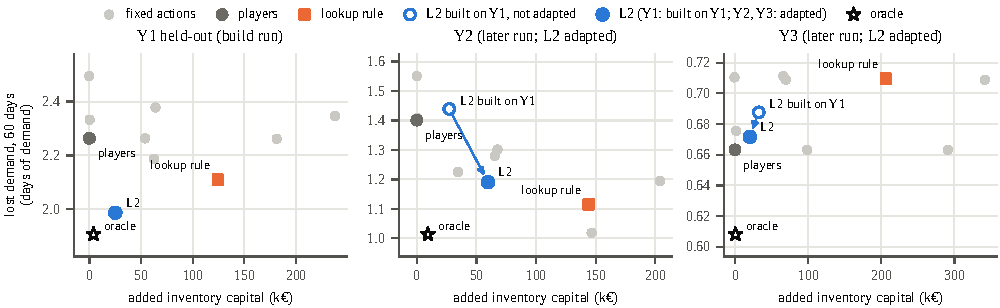
\includegraphics[width=\textwidth]{figures/fig5_l2_frontier.pdf}
\caption{L2: lost demand (all products, 60 days, in days of demand) against the added inventory capital of the
response. Left: build year, held-out episodes. Middle and right: other teams' years; the hollow circle is L2 built
on normal~2, the filled one L2 adapted with 400 target episodes (both on the same \num{1600} episodes).}
\label{fig:l2}
\end{figure*}

\textbf{L2.} On the held-out build-year episodes (Fig.~\ref{fig:l2}, left), the players lose 2.26 days of demand
and exceed the limit in 24.8\,\% of episodes; L2 loses 1.99 days (\num{-12}\,\%), exceeds the limit in 19.8\,\%,
acts in 34\,\% of episodes and adds 25\,k\euro{} of inventory, close to the oracle (1.91 days, 19.2\,\%). The
lookup rule spends 124\,k\euro{} and loses more (2.11 days). Little more is attainable: even the best action in
hindsight meets the limit in only 84\,\% of build-year episodes, because no lever repairs a long line stoppage.
On the other teams' years, L2 built on normal~2 is no better than the players (1.47 vs 1.43 days in fraud~2):
there, component buffers protect the other products, which never happened in the build year. Adapting L2 with 400
episodes of the target twin recovers a 15\,\% lower loss in fraud~2 (1.19 vs 1.40 days) at 60\,k\euro{}, against
147\,k\euro{} for the best fixed action. In fraud~3 there is little to gain, and the adapted L2 mostly does
nothing.

\begin{figure*}[t]
\centering
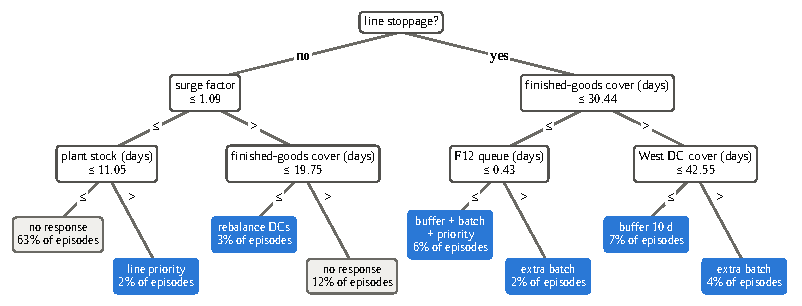
\includegraphics[width=\textwidth]{figures/fig6_tree.pdf}
\caption{The certified policy: L2 distilled into a depth-3 tree on features observed at the notice. Each leaf
shows the share of the independent certification episodes that reach it.}
\label{fig:tree}
\end{figure*}

\textbf{L3.} The tree (Fig.~\ref{fig:tree}) has eight leaves and six features. It first asks whether the line
has stopped; if so, it adds an extra F12 batch (with a component buffer and line priority when the F12 queue is
empty) or a component buffer, depending on finished-goods and DC cover. Otherwise it rebalances the DCs under a
surge above 1.09 with low finished-goods cover, gives F12 line priority when plant stock is high, and else does
nothing, which is the outcome in 75\,\% of episodes. It agrees with L2 on 77\,\% of
held-out build-year decisions, 69\,\% in fraud~2 and 56\,\% in fraud~3. The root split appears in all ten
bootstrap refits and the surge factor in every tree, but the lower splits vary (median agreement between refits
77\,\% in the build year, 54\,\% in fraud~3). The SHAP importance ranking of L1 (stoppage length, finished-goods
cover, North DC cover, surge factor first) is almost identical in every year (Spearman 0.96--0.99) although L1's
accuracy and coverage degrade: \emph{a stable explanation is not evidence that a model transfers}.

\begin{figure*}[t]
\centering
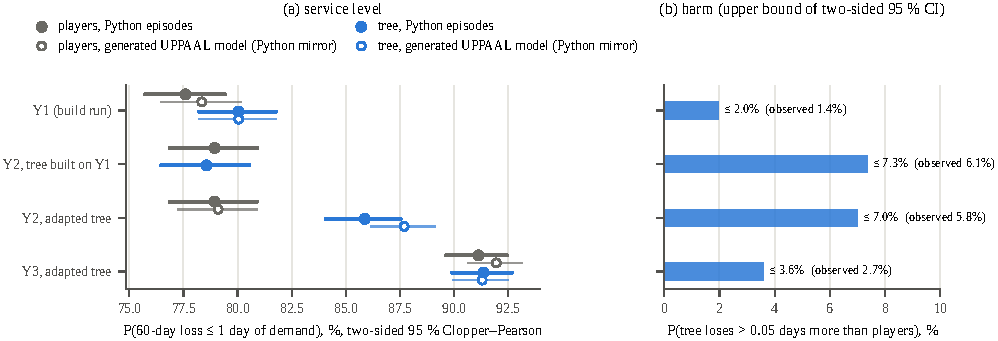
\includegraphics[width=\textwidth]{figures/fig7_certificates.pdf}
\caption{L4. (a) Probability that the 60-day loss stays within one day of demand, with 95\,\% Clopper--Pearson
intervals: filled markers on independent Python episodes, hollow markers from the generated UPPAAL model's own
random semantics. (b) Certified harm of the tree relative to the players' plan.}
\label{fig:cert}
\end{figure*}

\textbf{L4.} On the independent build-year sample (Fig.~\ref{fig:cert}), the players meet the limit in
77.6\,\% of episodes (certified $\ge$75.7\,\%), the tree in 80.0\,\% ($\ge$78.2\,\%) and the black-box L2 in
82.7\,\% ($\ge$80.9\,\%): the explanation costs about 2.7 points. The tree loses more than 0.05 days of demand above
the players' plan in 1.4\,\% of episodes (certified $\le$2.0\,\%). The tree built on normal~2 gives fraud~2 nothing ($\ge$77.0\,\% vs
$\ge$77.2\,\% for the players) and its certified harm rises to 7.1\,\%; the adapted tree certifies
$\ge$84.1\,\% against $\ge$76.9\,\%, with harm $\le$7.0\,\%. Against line stoppages no policy certifies more
than 21--49\,\%, a limit of the plant rather than of the AI. Executing the generated UPPAAL models with their own
random semantics gives 78.3 and 80.0\,\% in the build year and 87.7\,\% for the adapted tree in fraud~2, within
sampling error of the Python certificates.

\textbf{Robustness to the shipping rule.} Rebuilt on episodes generated with plain transfer replay, the pipeline
looks very different: the players lose about twice as much, shipping the stranded plant stock is the best action
in every year, and because that repair works for every team, coverage (89.5, 94.8, 94.4\,\%) and decision gains
(46, 58, 43\,\%) appear to transfer. The transfer failure reported above is therefore not created by the
corrected rule; the artefact hid it.

%% ------------------------------------------------------------------------------------------------------------
\section{Discussion}\label{sec:discussion}

\textbf{What can be trusted.} Within the population it was built for, the explainable policy improves the
service level with a certified bound and a certified low harm rate, uses the players' own levers, and does
nothing in three quarters of the cases. Outside that population, the conformal coverage, the decision value and
the certificate all degrade, and the certificate is what shows it. Explanation stability and SHAP rankings did
not. Two inexpensive repairs work: recalibrating the conformal margin on about 100 outcomes, and adapting the
decision layer with a few hundred episodes of the target's own twin. A twin per team, rather than one twin for
all, is the practical consequence.

\textbf{Twin validity matters more than model choice.} An unvalidated replay rule produced an AI that appeared
to transfer, for a reason that does not exist in the real game. Validation down to the replay rules is a
precondition for trustworthy AI on a twin.

\textbf{Limitations.} The data come from a business game, of one company, played by students; the evidence for
disruption severities is partly external and transferred as ratios; fraud~3 does not meet the pre-registered
validation verdict and the fraud years' DC stock is about two days of demand too high after the first month;
the other products are modelled at planning level; line stoppages cannot be mitigated with the available levers;
and the UPPAAL models still have to be executed in \texttt{verifyta} (the expected values are given above).
The tree is a learned policy certified by SMC, not a strategy synthesised by Stratego
\citep{david2015stratego}; synthesis over the same levers is a natural extension.

%% ------------------------------------------------------------------------------------------------------------
\section{Conclusion}

From the SAP records of three game years we built a supply-chain twin whose every part is backed by data and
validated on years it was not built on, generated it identically as a simulator and an UPPAAL model, and stacked
on it a predict--decide--explain--certify pipeline restricted to evidence-bounded disruptions and real levers.
The certified, readable policy improves service in its build year; transferred to another team it does not, and
the certificates say so. Recalibration and adaptation on the target twin restore coverage and value. Trustworthy
AI for disruption response therefore depends as much on the evidence behind the twin and on where guarantees are
evaluated as on the learning method.

% TODO(funding/acknowledgements)
\begin{ack}
The authors thank the authors of the open ERP dataset for releasing it.
\end{ack}

\bibliography{references}

\end{document}
